\documentclass{ximera}

\title{The art of Escher}

\begin{document}
\begin{abstract}
Here we look for connections between mathematics and art.
\end{abstract}
\maketitle

The famous artist M.C.\ Escher is known for drawing mind-boggling
art. Often there is a strong mathematical component to his art. One
thing that fascinated Escher was the question of how to depict an
infinitely repeating pattern in a finite space.

\begin{problem}
  Do you know of any methods for making the ``infinite finite'' from
  this class? If so, describe them.
\end{problem}

Around 1954, H.S.M.\ Coxeter (the famous geometer) learned of Escher's
work. As a source of inspiration, Coxeter sent Escher a picture
similar to this one:
\begin{image}
  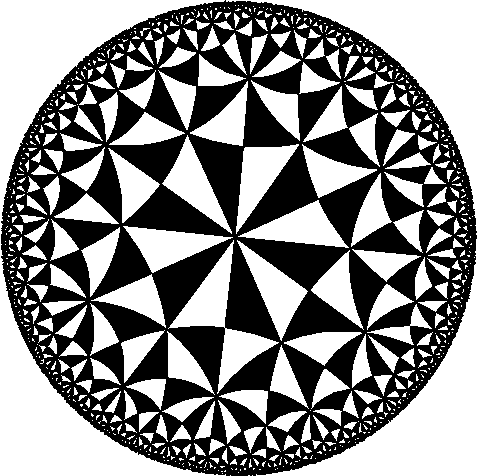
\includegraphics[width=3in]{inspiredCircleLimitIII.pdf}
\end{image}
Apparently Escher was ``shocked'' by this diagram, attempted to
reproduce it himself, and ran into some trouble. He then wrote to
Coxeter for assistance. After some time, Escher produced his own
versions, three of which are provided here for your viewing enjoyment:

\begin{image}
  \begin{array}{c}
  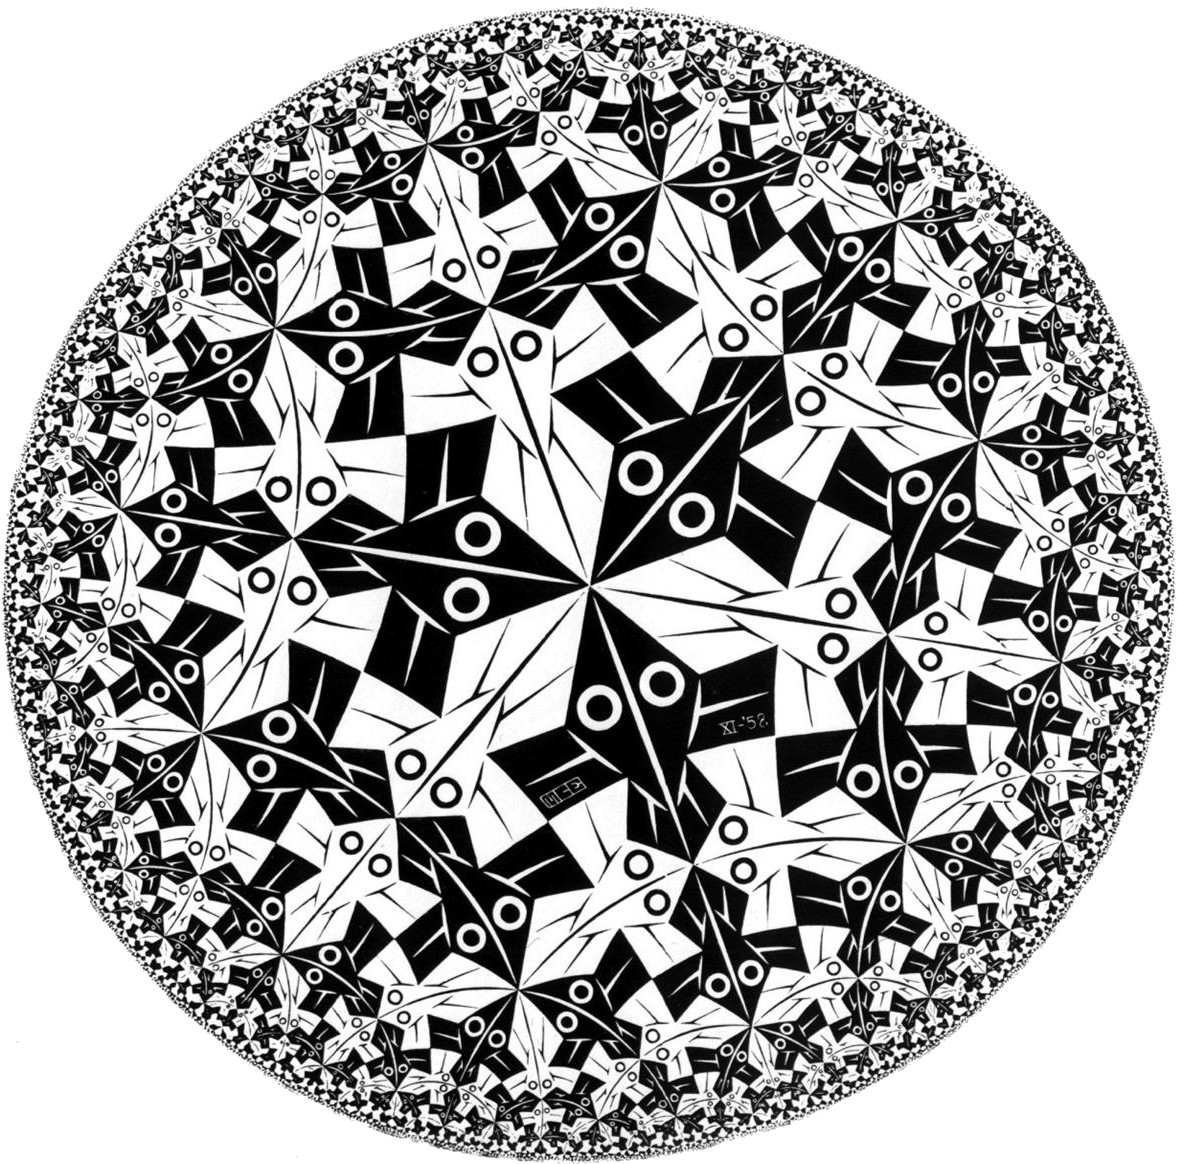
\includegraphics[width=3in]{circleLimitI.jpg}\\
  \text{\textit{Circle Limit I}. M.C.\ Escher, 1958}
  \end{array}
\end{image}

\begin{image}
  \begin{array}{c}
  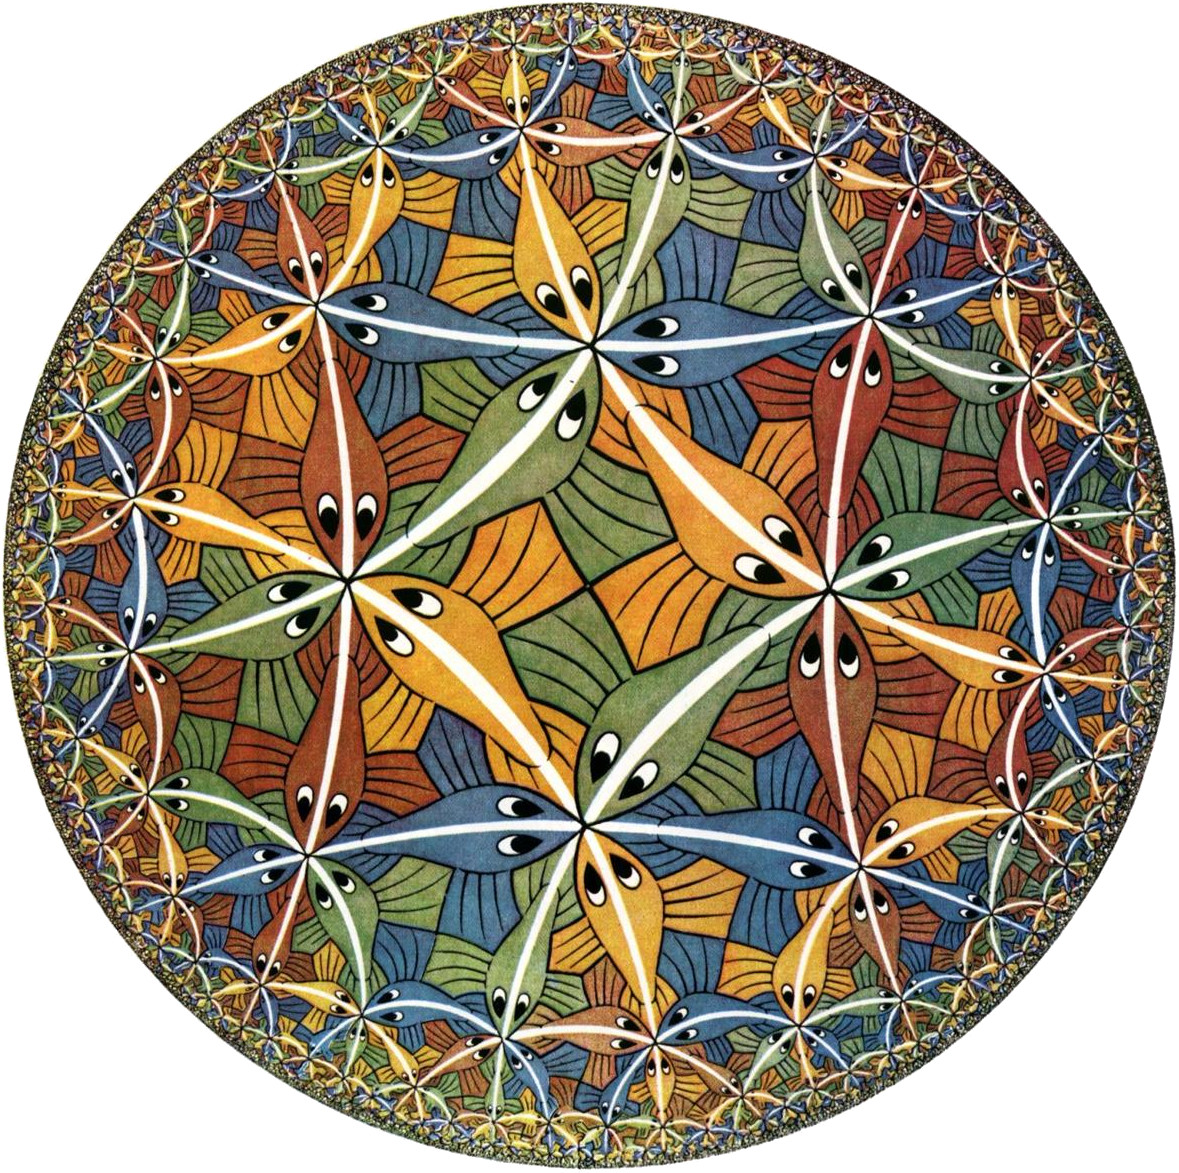
\includegraphics[width=3in]{circleLimitIII.jpg}\\
  \text{\textit{Circle Limit III}. M.C.\ Escher, 1959}
  \end{array}
\end{image}

\begin{image}
  \begin{array}{c}
  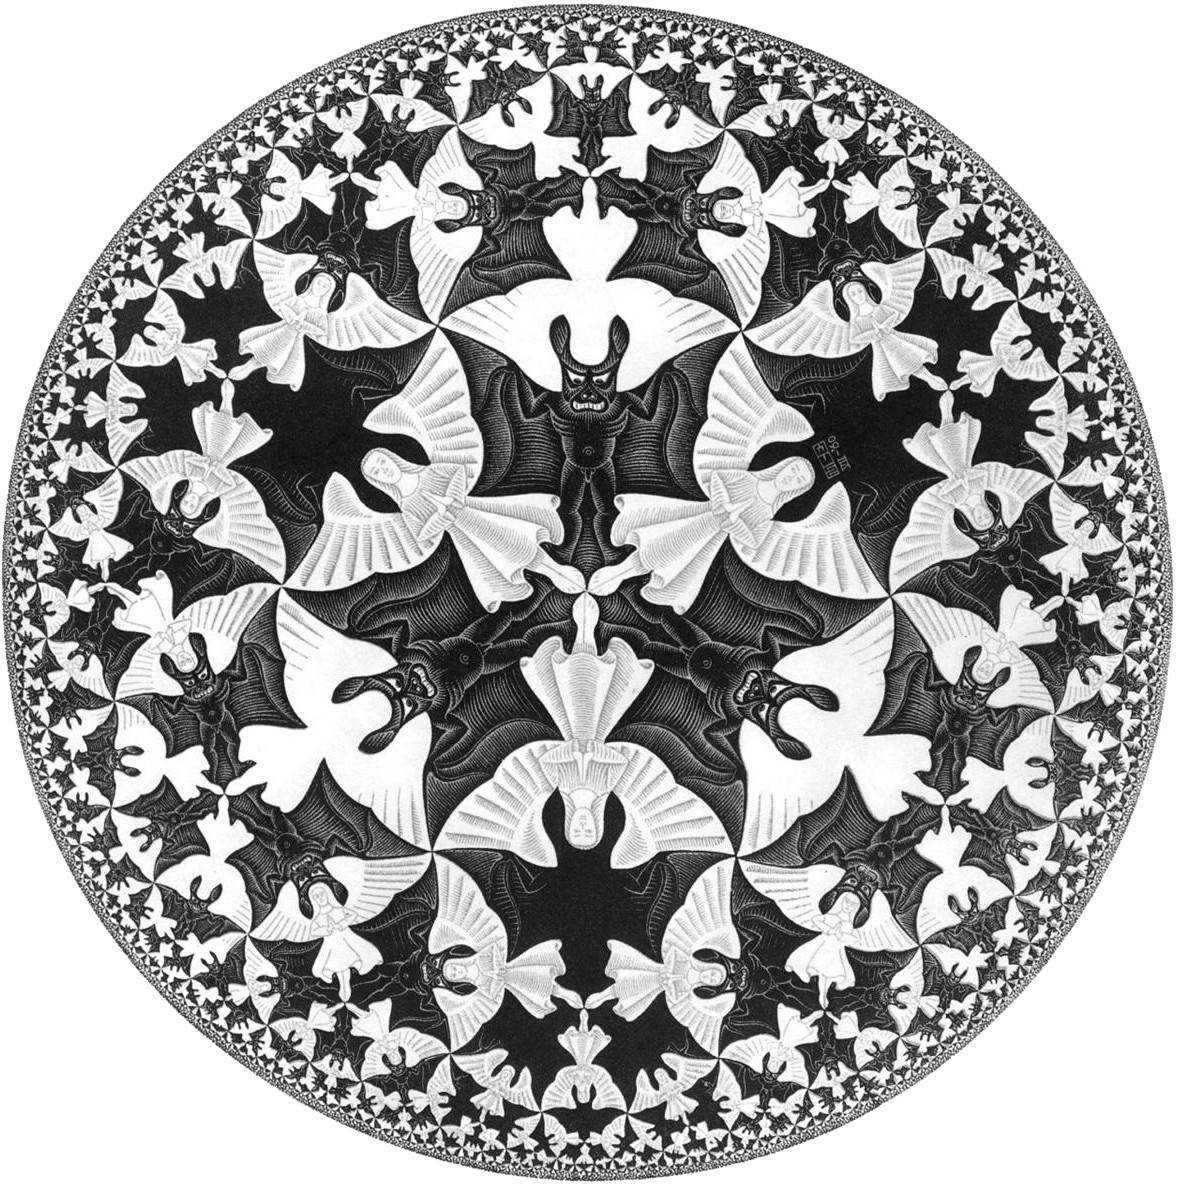
\includegraphics[width=3in]{circleLimitIV.jpg}\\
  \text{\textit{Circle Limit IV (Heaven and Hell)}. M.C.\ Escher, 1960}
  \end{array}
\end{image}

\break

\begin{problem}
Write down as many (mathematical) questions you can related to
Escher's work above. After you have your questions, label them as
``Level 1,'' ``Level 2,'' or ``Level 3'' where:
\begin{description}
\item[Level 1] Means you know the answer, or know exactly how to do this problem.
\item[Level 2] Means you think you know how to do the problem, or will
  be able to figure out how to do the problem.
\item[Level 3] Means you have no idea how to do the problem. 
\end{description}
\begin{freeResponse}
\end{freeResponse}
\end{problem}


\begin{problem}
  Someone once asked, can these ``distorted'' images be
  ``un-distorted.'' Answer ``no'' and support your answer with an
  argument. Answer ``yes'' and support your answer with an argument.
\end{problem}


\begin{problem}
  Building on ideas we learned in this course, what other sources of
  inspiration could you give to artists?
\end{problem}

\begin{problem}
Summarize the results and ideas from this \textbf{course}.
\begin{freeResponse}
\end{freeResponse}
\end{problem}


\end{document}
 
